
\begin{frame}{Podstawowe rozwiązania psuedo-rezystorów}


        \begin{figure}[H]
            \centering
            \includegraphics[scale = 0.6]{ch2/ntpr.pdf}

        \end{figure}
        \vspace{-5mm} %5mm vertical space
        % Różne topologie pseudo-rezystorów z niekontrolowaną wartością rezystancji zaimplementowane w przedwzmacniaczu ze sprzężeniem zmiennoprądowym.        
        \begin{alertblock}{Wady}
            \begin{itemize}
                \item stała rezystancja 
                \item brak możliwości regulacji częstotliwości granicznej
            \end{itemize}
        \end{alertblock}



\end{frame}

\begin{frame}{Podstawowe rozwiązania psuedo-rezystorów - regulowana wartość rezystancji}
    \begin{block}{}
        Regulacja częstotliowści granicznej
    \end{block}

    \begin{columns}
        \column{.58\textwidth}
        \hspace{-10mm} %5mm vertical space
        \begin{figure}[H]

            \includegraphics[scale = 0.6]{ch2/tpr.pdf}

        \end{figure}
        \column{.35\textwidth}
        % Różne topologie pseudo-rezystorów z kontrolowaną wartością rezystancji zaimplementowane w przedwzmacniaczu ze sprzężeniem zmiennoprądowym.
        \vspace{-5mm} \begin{alertblock}{}
        Zmieniające się napięcie panujące pomiędzy bramką a źródłem tranzystora w zależności od sygnału wejściowego
        \end{alertblock}
        \vspace{5mm} 
        \begin{exampleblock}{}
            Zachowanie stałego napięcia pomiędzy bramką, a źródłem niezależnie od sygnału wejsciowego 

        \end{exampleblock}
    \end{columns}


\end{frame}







\begin{frame}{Analiza stałoprądowa}

        
    \vspace{-1em}


    \begin{columns}
        \column{.48\textwidth}
         \begin{alertblock}{}
            \begin{figure}[H]
                \includegraphics[scale=0.8]{ch3/ptune.pdf}
            \end{figure}
            \end{alertblock}
        \column{.48\textwidth}
        \begin{exampleblock}{}
            \begin{figure}[H]
                \includegraphics[scale=0.8]{ch3/pvgs.pdf}
            \end{figure}

        \end{exampleblock}
    \end{columns}

\vspace{-0.5em}
    \begin{columns}
        \column{.48\textwidth}
        \begin{figure}[H]
            \centering
            \includegraphics[scale = 0.7]{scripts/tmp/pseudoresistors_IV.pdf}
                \end{figure}
        \column{.48\textwidth}
        \begin{figure}[H]
            \centering
            \includegraphics [scale = 0.7]{scripts/tmp/pseudoresistors_R.pdf}
        \end{figure}
    \end{columns}


\end{frame}

\begin{frame}{Architektura wzmacniacza neuronowego wykorzystującego sprzężenie zmiennoprądowe w różnych implementacjach pseudo-rezystorów}
    \begin{columns}[t]
        \column{.4\textwidth}
        \begin{alertblock}{Zmienne napięcia na bramce -- $variable-V_{gs}$}
            \begin{figure}[H]
                \centering
                \includegraphics[scale = 0.75]{ch3/fig1-ac_standard.pdf}
            \end{figure}
        \end{alertblock}



        \column{.4\textwidth}
        \begin{exampleblock}{Słałe napięcia na bramce -- $fixed-V_{gs}$}
            \begin{figure}[H]
                \centering
                \includegraphics[scale = 0.75]{ch3/fig1-ac_work_simplicite}
            \end{figure}
        \end{exampleblock}

    \end{columns}
\end{frame}

\begin{frame}{Analiza Transient sprzężenia AC}
    \begin{block}{Ustawienia symulacji}
\begin{itemize}
    \item Czeęstotliwość graniczna dla sprzężenia AC $\SI{\sim 1}{\hertz}$
    \item $\mathrm{THD} = \frac{\sqrt{\sum_{n=2}^{+\infty} U_k^2}}{U_1}$
\end{itemize}
    \end{block}


    \begin{columns}
        \column{.48\textwidth}
        \begin{figure}[H]
            \centering
            \includegraphics[scale = 0.7]{scripts/tranTHDAmp/tranTHDAmp_ner.pdf}
        \end{figure}
        \column{.48\textwidth}
        \begin{figure}[H]
            \centering
            \includegraphics[scale = 0.7]{scripts/tranTHDAmp/tranTHDAmp_pr_sim.pdf}
        \end{figure}
    \end{columns}

\end{frame}



\begin{frame}{Projekt przedwzmacniacza z modelem pseudo-rezystora w technologii $\SI{180}{\nano\metre}$  XFAB}
    \begin{figure}[H]
        \centering
        \includegraphics[scale=1.0]{ch3/pseudo-lay.pdf} 

    \end{figure}


\end{frame}

\begin{frame}{Wpływ pojemnościowych prądów bramki pseudo-rezystorów na zniekształcenia  w technologii $\SI{180}{\nano\metre}$}
    \vspace{-5mm} %5mm vertical space

    \begin{columns}
        \column{.3\textwidth}
        \begin{figure}[H]

            \includegraphics[trim={0 0.25cm 0 0.25cm}, clip, scale = 0.6]{scripts/tmp/IdsA.pdf}

        \end{figure}
        \column{.3\textwidth}
        \begin{figure}[H]

            \includegraphics[trim={0 0.25cm 0 0.25cm}, clip, scale = 0.6]{scripts/tmp/IdsB.pdf}

        \end{figure}
        \column{.3\textwidth}
        \begin{figure}[H]

            \includegraphics[trim={0 0.25cm 0 0.25cm}, clip, scale = 0.6]{scripts/tmp/IgbA.pdf}

        \end{figure}

    \end{columns}
    \vspace{-10mm} %5mm vertical space
    \begin{columns}
        \column{.3\textwidth}
        \begin{figure}[H]

            \includegraphics[trim={0 0.25cm 0 0.25cm}, clip, scale = 0.6]{scripts/tmp/IgbB.pdf}

        \end{figure}
        \column{.3\textwidth}
        \begin{figure}[H]

            \includegraphics[trim={0 0.25cm 0 0.25cm}, clip, scale = 0.6]{scripts/tmp/vOut.pdf}

        \end{figure}
        \column{.3\textwidth}
        \begin{figure}[H]

            \includegraphics[trim={0 0.25cm 0 0.25cm}, clip, scale = 0.6]{scripts/tmp/Igb_diff.pdf}

        \end{figure}

    \end{columns}
        



\end{frame}


\begin{frame}{Skalowanie zniekształceń z powierzchnią bramki i grubością tlenku tranzystorów tworzących pseudo-rezystory}
    \begin{columns}
        \column{.48\textwidth}
        \begin{block}{Powierzchnia bramki -- technologia $\SI{180}{\nano\metre}$ }
            \begin{figure}[H]
                \centering
                \includegraphics[scale = 0.7]{scripts/analyseTran/analyseTranSize.pdf}
            \end{figure}
        \end{block}

        \column{.48\textwidth}
        \begin{block}{Zależnosć od technologii}
            \begin{figure}[H]
                \centering
                \includegraphics[scale = 0.7]{scripts/analyseTran/analyseTranTechnology.pdf}
            \end{figure}
        \end{block}


    \end{columns}

\end{frame}

\begin{frame}{Szumy}
    \vspace{-5mm} %5mm vertical space

    \begin{columns}
    \column{.3\textwidth}
    \begin{figure}[H]
        \centering
        \includegraphics[scale=0.5]{ch2/conceptAC_Harrison.pdf} 
    \end{figure}
        \column{.3\textwidth}
        \begin{figure}[H]
            \centering
            \includegraphics[scale = 0.5]{scripts/tmp/fig3_R1.pdf}
        \end{figure}
        \column{.3\textwidth}
        \begin{figure}[H]
            \centering
            \includegraphics[scale = 0.5]{scripts/tmp/fig3_R2.pdf}
        \end{figure}
    \end{columns}

    \vspace{-5mm} %5mm vertical space


    \begin{columns}
        \column{.3\textwidth}
        \begin{figure}[H]
            \centering
            \includegraphics[scale=0.5]{scripts/noiseOutResistors/fig1_R1.pdf}
        \end{figure}
        \column{.3\textwidth}
        \begin{figure}[H]
            \centering
            \includegraphics[scale=0.5]{scripts/noiseOutResistors/fig2.pdf}
        \end{figure}
    \end{columns}


\end{frame}


\begin{frame}{Wpływ pojemności wejściowych na szumy i zniekształcenia}
    \begin{figure}[H]
        \centering
        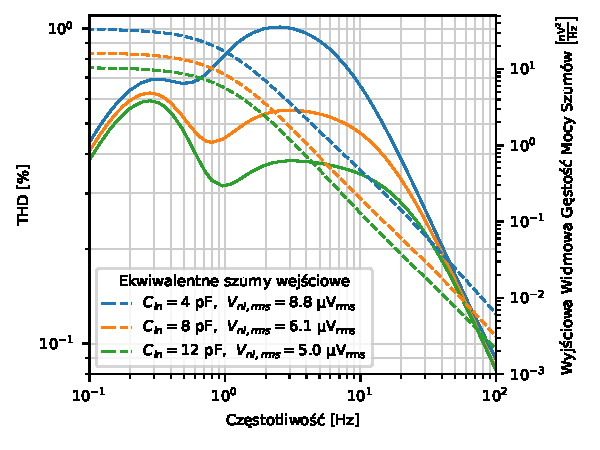
\includegraphics{scripts/tmp/thd_C_in.pdf} 
    \end{figure}

\end{frame}
